\documentclass[aspectratio=169,11pt,hyperref={colorlinks=true}]{beamer}
\usetheme{boxes}
\setbeamertemplate{navigation symbols}{}
\definecolor{ibm}{RGB}{70,107,176}
\setbeamercolor{titlelike}{fg=ibm}
\setbeamercolor{structure}{fg=ibm}
\hypersetup{colorlinks,urlcolor=ibm}
\setbeamertemplate{footline}[frame number]
% Inserting graphics
\usepackage{graphicx}
% Side-by-side figures, etc
\usepackage{subfigure}
% Code snippits
\usepackage{listings}

\usepackage{lmodern}
% Color stuff
\usepackage{color}
\usepackage{amsmath}
\usepackage{amssymb}
\usepackage{empheq}
\usepackage[braket, qm]{qcircuit}
\usepackage{tikz}
\usepackage{gensymb}
\newcommand\RBox[1]{%
  \tikz\node[draw,rounded corners,align=center,] {#1};%
}
\usepackage{hyperref}
%\usecolortheme{buzz}
%\usecolortheme{wolverine}
%\usetheme{Boadilla}
\usepackage[T1]{fontenc}

\definecolor{mygreen}{rgb}{0,0.6,0}
\definecolor{mygray}{rgb}{0.5,0.5,0.5}
\definecolor{mymauve}{rgb}{0.58,0,0.82}

\lstset{%
  backgroundcolor=\color{white},   % choose the background color; you must add \usepackage{color} or \usepackage{xcolor}
  breakatwhitespace=false,         % sets if automatic breaks should only happen at whitespace
  breaklines=true,                 % sets automatic line breaking
  captionpos=b,                    % sets the caption-position to bottom
  commentstyle=\color{ibm},  % comment style
  extendedchars=true,              % lets you use non-ASCII characters; for 8-bits encodings only, does not work with UTF-8
  keepspaces=true,                 % keeps spaces in text, useful for keeping indentation of code (possibly needs columns=flexible)
  keywordstyle=\color{blue},       % keyword style
%  otherkeywords={*,...},           % if you want to add more keywords to the set
  numbersep=5pt,                   % how far the line-numbers are from the code
  numberstyle=\tiny\color{mygray}, % the style that is used for the line-numbers
  rulecolor=\color{black},         % if not set, the frame-color may be changed on line-breaks within not-black text (e.g. comments (green here))
  showspaces=false,                % show spaces everywhere adding particular underscores; it overrides 'showstringspaces'
  showstringspaces=false,          % underline spaces within strings only
  showtabs=false,                  % show tabs within strings adding particular underscores
  stringstyle=\color{ibm},   % string literal style
}


\setbeamerfont{caption}{series=\normalfont,size=\fontsize{6}{8}}
\setbeamertemplate{caption}{\raggedright\insertcaption\par}

\setlength{\abovecaptionskip}{0pt}
\setlength{\floatsep}{0pt}

\author[Matthew Treinish]{%
    \texorpdfstring{%
        \centering
        Matthew Treinish\\
        Software Engineer - IBM Research\\
        \href{mailto:mtreinish@kortar.org}{mtreinish@kortar.org}\\
        \texttt{mtreinish on Freenode}\\
        \href{https://github.com/mtreinish/quantum-compilers}{https://github.com/mtreinish/quantum-compilers}
   }
   {Matthew Treinish}
}
\date{January 17, 2020}

\title{Building a Compiler for Quantum Computers}
\begin{document}

\titlepage
\section{How to Programs are written for Quantum Computers}
\subsection{Quantum Circuits}
\begin{frame}
    \frametitle{Quantum Circuits}
    
\end{frame}
\subsubsection{OpenQASM}
\begin{frame}
    \frametitle{OpenQASM}
    \begin{columns}
        \column{0.5\textwidth}
            \lstinputlisting{bell.qasm}
        \column{0.5\textwidth}
            \begin{equation*}
                \Qcircuit @C=1.0em @R=0.0em @!R {
            	 	\lstick{ q_{0} : \ket{0} } & \gate{H} & \ctrl{1} & \meter & \qw & \qw & \qw\\
            	 	\lstick{ q_{1} : \ket{0} } & \qw & \targ & \qw & \meter & \qw & \qw\\
            	 	\lstick{c_{0}: 0} & \cw & \cw & \cw \cwx[-2] & \cw & \cw & \cw\\
            	 	\lstick{c_{1}: 0} & \cw & \cw & \cw & \cw \cwx[-2] & \cw & \cw\\
            	}
            \end{equation*}
    \end{columns}
\end{frame}
\subsection{Pulse}
\begin{frame}
    \frametitle{Pulse Level Programming}
    \begin{columns}
        \column{0.5\textwidth}
            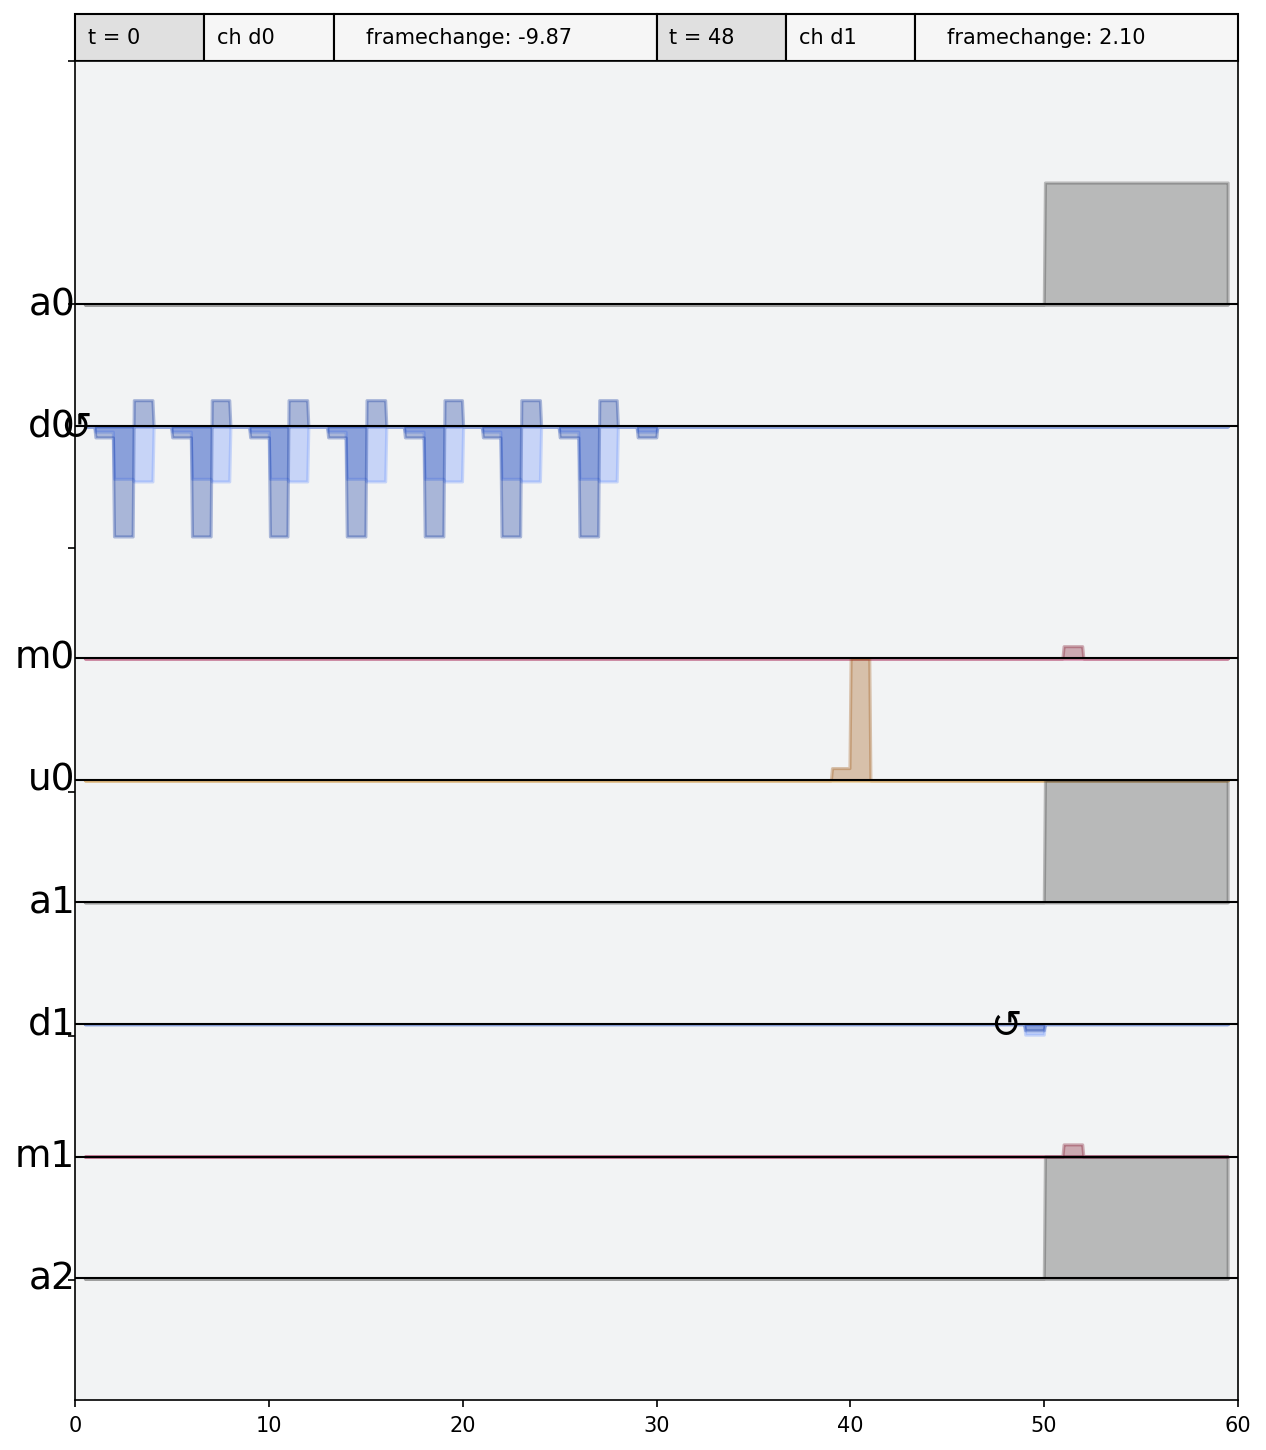
\includegraphics[width=\textwidth]{bell-sched.png}
        \column{0.5\textwidth}
            \begin{equation*}
                \Qcircuit @C=1.0em @R=0.0em @!R {
                    \lstick{ q_{0} : \ket{0} } & \gate{H} & \ctrl{1} & \meter & \qw & \qw & \qw\\
                    \lstick{ q_{1} : \ket{0} } & \qw & \targ & \qw & \meter & \qw & \qw\\
                    \lstick{c_{0}: 0} & \cw & \cw & \cw \cwx[-2] & \cw & \cw & \cw\\
                    \lstick{c_{1}: 0} & \cw & \cw & \cw & \cw \cwx[-2] & \cw & \cw\\
                }
            \end{equation*}
    \end{columns}

\end{frame}

\section{Constraints for Running on Quantum Computers}
\subsection{Qubit Connectivity}
\begin{frame}
    \frametitle{Qubit Connectivity}
    \begin{columns}
        \column{.5\textwidth}
            \begin{itemize}
                \item Qubits in a device have limited connectivity
                \item For multi-qubit gates this means we can only run them
                    between those qubits
                \item Need to use SWAP gates to move state around
            \end{itemize}
        \column{.5\textwidth}
            \centering
            \only<1>{\textbf{IBM Q 5 Yorktown}\\}
            \only<1>{\includegraphics[width=\textwidth]{ibmqx2-labeled.png}}
            \only<2>{\textbf{IBM Q 53 Rochester Coupling Map}\\}
            \only<2>{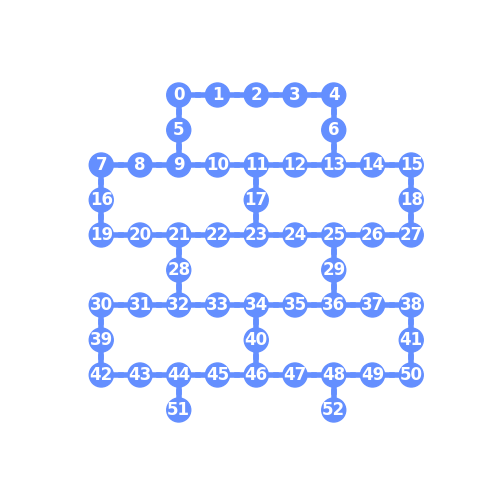
\includegraphics[width=\textwidth]{rochester_map.png}}
    \end{columns}
\end{frame}
\begin{frame}
    \frametitle{Mapping}
    \begin{equation*}
        \Qcircuit @C=1.0em @R=0.0em @!R {
    	 	\lstick{ {q0}_{0} : \ket{0} } & \gate{H} & \qw & \ctrl{4} & \gate{H} & \qw & \qw & \qw & \qw & \qw\\
    	 	\lstick{ {q0}_{1} : \ket{0} } & \gate{H} & \qw & \qw & \ctrl{3} & \gate{H} & \qw & \qw & \qw & \qw\\
    	 	\lstick{ {q0}_{2} : \ket{0} } & \gate{H} & \qw & \qw & \qw & \ctrl{2} & \gate{H} & \qw & \qw & \qw\\
    	 	\lstick{ {q0}_{3} : \ket{0} } & \gate{H} & \qw & \qw & \qw & \qw & \ctrl{1} & \gate{H} & \qw & \qw\\
    	 	\lstick{ {q0}_{4} : \ket{0} } & \gate{X} & \gate{H} & \targ & \targ & \targ & \targ & \gate{H} & \qw & \qw\\
    	 }
    \end{equation*}

    \begin{equation*}
    \Qcircuit @C=1.0em @R=0.0em @!R {
	 	\lstick{ {q}_{0} : \ket{0} } & \gate{H} & \qswap & \qw & \qw & \qw & \qw & \qw & \qswap & \qw & \qw & \qw & \qw & \qw\\
	 	\lstick{ {q}_{1} : \ket{0} } & \gate{H} & \qw & \qw & \qw & \qswap & \qw & \qw & \qw & \qw & \qw & \qw & \qw & \qw\\
	 	\lstick{ {q}_{2} : \ket{0} } & \gate{H} & \qswap \qwx[-2] & \ctrl{2} & \gate{H} & \qswap \qwx[-1] & \ctrl{2} & \gate{H} & \qswap \qwx[-2] & \ctrl{2} & \gate{H} & \qw & \qw & \qw\\
	 	\lstick{ {q}_{3} : \ket{0} } & \gate{H} & \qw & \qw & \qw & \qw & \qw & \qw & \qw & \qw & \ctrl{1} & \gate{H} & \qw & \qw\\
	 	\lstick{ {q}_{4} : \ket{0} } & \gate{X} & \gate{H} & \targ & \qw & \qw & \targ & \qw & \qw & \targ & \targ & \gate{H} & \qw & \qw\\
	 }
\end{equation*}

\begin{equation*}
    \Qcircuit @C=1.0em @R=0.0em @!R {
	 	\lstick{ {q}_{0} : \ket{0} } & \gate{X} & \gate{H} & \targ & \qswap & \gate{H} & \qw & \qw & \qw & \qw & \qw & \qw\\
	 	\lstick{ {q}_{1} : \ket{0} } & \gate{H} & \qw & \qw & \qw & \qw & \qw & \qw & \ctrl{1} & \gate{H} & \qw & \qw\\
	 	\lstick{ {q}_{2} : \ket{0} } & \gate{H} & \qswap \qwx[2] & \ctrl{-2} & \qswap \qwx[-2] & \targ & \qw & \targ & \targ & \gate{H} & \qw & \qw\\
	 	\lstick{ {q}_{3} : \ket{0} } & \gate{H} & \qw & \qw & \qw & \ctrl{-1} & \gate{H} & \qw & \qw & \qw & \qw & \qw\\
	 	\lstick{ {q}_{4} : \ket{0} } & \gate{H} & \qswap & \qw & \qw & \qw & \qw & \ctrl{-2} & \gate{H} & \qw & \qw & \qw\\
	 }
\end{equation*}


\end{frame}
\subsection{Other Device Characteristics}
\begin{frame}
    \frametitle{Basis Gates}

\end{frame}
\begin{frame}
    \frametitle{Unrolling}

\end{frame}
\subsection{Noise}
\begin{frame}

\end{frame}

\section{Qiskit's Compiler}
\begin{frame}
    \frametitle{Qiskit Terra}
    \begin{columns}
          \column{.5\textwidth}
             \begin{itemize}
                  \item Is the base layer for working with quantum computers provides interface to hardware and simulators
                  \item Provides an SDK for working with quantum circuits
                  \item Compiles circuits to run on different backends
                  \item Designed to be backend agnostic and work with any
                      quantum hardware or simulator
                  \item Written in Python
             \end{itemize}
          \column{.5\textwidth}
              \centering
              \colorbox{black}{
\includegraphics[width=.5\textwidth]{qiskit-terra-logo.png}}
      \end{columns}
  \end{frame}

\subsection{The DAG}
\begin{frame}
    \frametitle{The DAG}
        \begin{columns}
            \column{0.5\textwidth}
                \begin{itemize}
                    \item Compiler represents circuits as a DAG
                    \item Each node in the DAG is an operation, an input, or
                          an output
                    \item Each edge corresponds to a qubit or classical bit
                \end{itemize}
            \column{0.5\textwidth}
                \centering
                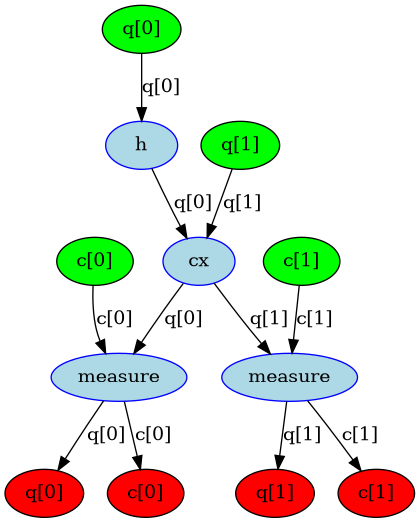
\includegraphics[width=0.75\textwidth]{bell-dag.png}
        \end{columns}
\end{frame}
\begin{frame}
    \frametitle{Pass Manager}
    \begin{columns}
        \column{0.5\textwidth}

        \column{0.5\textwidth}
            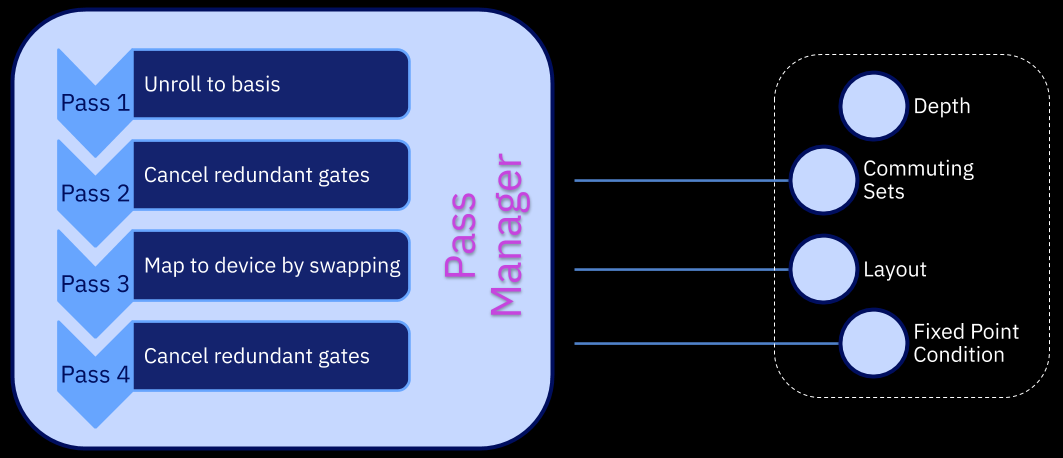
\includegraphics[width=\textwidth]{passmanager.png}
    \end{columns}
\end{frame}
\subsection{Preset Pass Managers}
\section{Passes}
\begin{frame}
    \frametitle{Types of passes}
    \begin{columns}
        \column{.45\textwidth}
            \textbf{Transformation Passes} \\
            \begin{itemize}
                \item Can alter the DAG during execution
                \item Read-only access to the property set
                \item
            \end{itemize}
        \column{.45\textwidth}
            \textbf{Analysis Passes} \\
            \begin{itemize}
                \item Can alter the property set
                \item Read-only access to the DAG
            \end{itemize}
    \end{columns}
\end{frame}
\subsection{Unroller}
\begin{frame}
    \frametitle{The Unroller}
\end{frame}
\subsection{Gate Cancellation}
\subsubsection{Optimize 1Q operations}
\begin{frame}
    \frametitle{Optimize 1Q Operations}
\end{frame}
\subsubsection{Consolidate Blocks}
\begin{frame}

\end{frame}
\subsection{Device Mapping}

\section{Conclusions}
\subsection{Quantum Volume}
\begin{frame}
    \frametitle{Quantum Volume\footnotemark[1]}

    \vspace{3em}
    \footnotetext[1]{https://arxiv.org/abs/1811.12926}
\end{frame}
\begin{frame}
    \frametitle{Conclusions}
    \begin{itemize}
        \item similar but different
    \end{itemize}
\end{frame}

\section{Questions?}
\begin{frame}
\frametitle{Where to get more information}
    \begin{itemize}
        \item These Slides: \href{https://github.com/mtreinish/quantum-compilers}{https://github.com/mtreinish/quantum-compilers}
        \item Qiskit: \href{https://qiskit.org/}{https://qiskit.org/}
        \item Qiskit Terra on Github: \href{https://github.com/Qiskit/qiskit-terra}{https://github.com/Qiskit/qiskit-terra}
        \item IBM Q Experience: \href{https://quantum-computing.ibm.com}{https://quantum-computing.ibm.com}
        \item Tutorials on Quantum Computing and Qiskit: \href{https://github.com/Qiskit/qiskit-tutorials}{https://github.com/Qiskit/qiskit-tutorials}
    \end{itemize}
\end{frame}

\section{Backup Slides}
\begin{frame}[noframenumbering]
    \frametitle{BACKUP SLIDES}
\end{frame}

\end{document}
